\namedsubsection{QDX}{J}
Das Datenaustauschformat für Qualitätsdaten QDX ist eine vom Verband der Automobilindustrie e. V. (VDA) seit 2004 entwickeltes Format basierend auf den damals üblichen Kerntechnologien SOAP und XML. Es dient vor allem dazu Qualitätsdaten zwischen Kunden und Lieferanten der Automobilbranche zu vereinheitlichen. Dies soll es ermöglichen den Aufwand für die Kommunikation zu reduzieren.
Nachfolgend schlüsseln wir den groben Aufbau des Formates auf und nennen verwendete Technologien, Modelle und weitere für das Verständnis wichtige Informationen.

\subsubsection*{Aufbau}
Die meisten Elemente des Formates sind unidirektional ausgelegt. Das bedeutet, dass einige Elemente ausschließlich ausgehend vom Kunden (Beanstandung) oder vom Lieferanten (Fähigkeitsuntersuchung) an die Gegenseite übermittelt wird. In der Regel können diese Elemente um Anhänge jedweder Art ergänzt werden (z. B. Videos, PDFs, etc.).

% Technologie
Die Daten selbst liegen in XML-Form vor und werden auf Basis von SOAP übertragen. Hierbei macht es keinen Unterschied ob die Übertragung über HTTP oder TCP/UDP stattfindet. Daten die als XML vorliegen haben einige Vorteile hinsichtlich des verfügbaren Toolings. So können die Daten per XSD validiert werden oder über XST in andere Formate umgewandelt werden. Im Falle von QDX liegen die Schema-Dateien bereits vor.
Zusätzlich liegt eine WSDL für den Complaint-Prozess vor. WSDL dienen als Beschreibung der Möglichkeiten eines Services.
Kommen Webservices zum Einsatz wird als Übertragungsprotokoll HTTPS empfohlen und eine Authentifizierung findet über den Authorization Header (Basic) statt in dem der Username und das Passwort übertragen werden. Im anderen Fall kommt OFTP zum Einsatz.

% Modelle
Das QDX Format kommt mit zahlreichen vordefinierten Elementen. Im Kontext von QDX wird aber häufig auch von Dokumenten gesprochen, weil die Datenmodelle üblicherweise den schriftlichen Verkehr zwischen Kunden und Lieferanten der Automobilindustrie im Qualitätsmanagement nachempfunden sind. Zwei besonders wichtige Dokumente werden hier mit einer kurzen Beschreibung aufgelistet.

\begin{description}
    \item[Beanstandungsmeldung] Mit Beanstandungsmeldungen werden Lieferanten vom Kunden auf Qualitätsmängel ihrer Lieferungen hingewiesen. Diese enthalten insbesondere Informationen über etwaige Sachmängel.
    \item[8D-Report] Mit einem 8D-Report werden dem Kunden Informationen darüber ausgestellt wie die Beanstandung nach der 8D-Methodik behoben werden soll. Die 8D-Methodik wiederum beschreibt einen lösungsorientierten Prozess um vorhandene Qualitätsprobleme dauerhaft auszumerzen.
\end{description}

% Prozesse
In QDX unterscheidet man zwischen aktiver und passiver Kommunikation. Im Fall von aktiver Kommunikation wird das Protokoll OFTP verwendet und im anderen Fall übliche Webservices über HTTP/HTTPS.

\begin{figure}[!h]
\centering
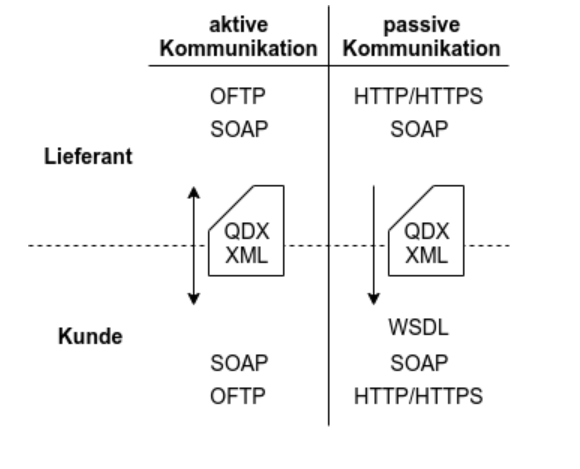
\includegraphics[width=8cm]{images/0x_requirement_analysis/qdx_communication_process}
\caption{QDX Communication Process}
\end{figure}

Das muss im Vorfeld auf beiden Seiten geklärt werden. Passive Kommunikation meint hierbei, dass der Schritt für die Initiierung stets auf der Lieferantenseite stattfindet\footnote{Quelle 2, S. 29: “Bei der „passiven“ Kommunikation ist also immer der Lieferant dafür verantwortlich, dass er die Daten des Kunden erhält und dass seine Daten an den Kunden übermittelt werden. Der Lieferant ist somit sowohl in der „Bring-“ als auch in der „Holschuld“.”}. Zu beachten ist hierbei, dass damit auch Veränderungen im Ablauf der Kommunikation entstehen. Insbesondere bedeutet es das zusätzliche Elemente für die Kommunikation benötigt werden (z. B. QDXComplaintList).
Bestimmte Dokumenteneingänge wie Beanstandungsmeldungen oder 8D-Reports müssen grundsätzlich von der Gegenseite über Acknowledge-Antworten bestätigt werden.
Nachfolgend werden Beispielabläufe für Beanstandungen in der aktiven sowie passiven Varianten dargestellt.

\begin{description}
\item [Variante aktive Kommunikation (über OFTP2)]\hfill
    \begin{enumerate}
        \item Lieferant <—QDXComplaint— Kunde
        \item Lieferant —QDXAcknowledgeComplaint—> Kunde
    \end{enumerate}
\item [Variante passive Kommunikation (über HTTP/HTTPS)]\hfill
    \begin{enumerate}
        \item Lieferant —QDXComplaintListRequest—> Kunde
        \item Lieferant <—QDXComplaintList— Kunde
        \item Lieferant —QDXComplaintRequest—> Kunde
        \item Lieferant <—QDXComplaint— Kunde
        \item Lieferant —QDXComplaintAcknowledgment—> Kunde
    \end{enumerate}
\end{description}

% Aufbau Datenpaket

% \begin{figure}[!h]
% \centering
% 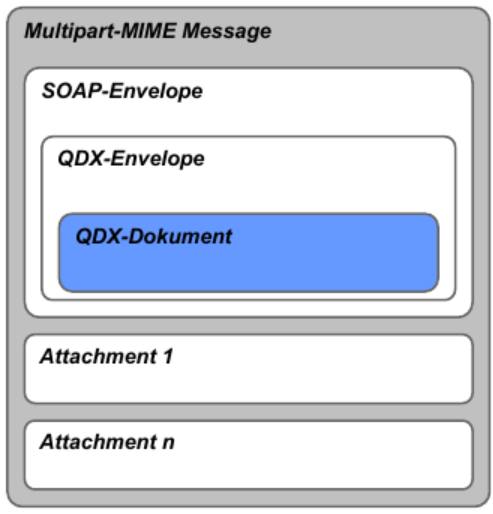
\includegraphics[width=7cm]{images/0x_requirement_analysis/qdx_message_structure.png}
% \caption{QDX Message Structure}
% \end{figure}

\subsubsection*{Vorteile}
\begin{itemize}
    \item Standard aus Verband der Automobilbranche e. V., es wird von vielen großen Autoherstellern und deren direkten Lieferanten genutzt
    \item Schema zur Validierung der Daten bereits verfügbar
    \item WSDL für den Complaint-Prozess enthalten
    \item Ausgereiftes Tooling für XML
\end{itemize}

\subsubsection*{Nachteile}
\begin{itemize}
    \item Technischer Unterbau wurde im Jahr 2005 entworfen
    \item Für einen reibungslosen Vorgang sind Abstimmungen mit den Lieferantensystemen nötig und für jeden Geschäftsprozess extra festzulegen (Leistungsmerkmale wie maximal zulässige Latenz, aktive/passive Kommunikation, etc.), denn diese werden von QDX nicht vorgegeben
    \item Unterschiedliche Kommunikationsweisen (aktiv/passiv) des Datenaustausches erfordern unterschiedliche Implementationen
    \item Die passive Kommunikation ist längst nicht so versatil wie die aktive Variante, weil ausschließlich die Lieferanten-Seite für die Übertragung und dem Beziehen von Daten verantwortlich ist
    \item Die Webservice-Variante erlaubt nur die unsichere Authentifizierung über Basic Authentication Header
    \item Für OFTP existieren vorwiegend kommerzielle Clients
    \item Lizenzgebühren für Nutzung in Softwareprodukte
    \item Einarbeitung in OFTP nötig
\end{itemize}

% Empfehlung
Da QDX beim aktuellen Kunden gegenwärtig nicht in Verwendung ist, wurde aus Gründen der Komplexität vorerst auf eine Einbindung verzichtet.
Falls es irgendwann doch dazu kommt, sollte man sich auf die Bestandteile des Formates konzentrieren die auch tatsächlich im operativen Geschäft beim Kunden benutzt werden.
Vermutlich am Ehesten alles bezogen auf Complaint-Prozesse plus 8D Reports.
Da sich die Dokumente an den realen Schriftverkehr bei Qualitätsbeanstandungen orientierte, könnte es Sinn ergeben sich bei der eigenen Modellierung durch die Überlegungen aus QDX inspirieren zu lassen.